\section{ODE Model}
\label{sec-ode}
In this section, we use the simple SIR ODE model to fit the COVID-19 data in Singapore as a supplement to our complicated agent-based model and to get a basic idea about the ranges of the parameters.
\subsection{Background and domain research}
First we plot the daily confirmed data before and after vaccination to have an intuitive understanding on the outbreaks of COVID-19 in Singapore (Figure \ref{sir0} and Figure \ref{sir1}).

\begin{figure}
	\centering
	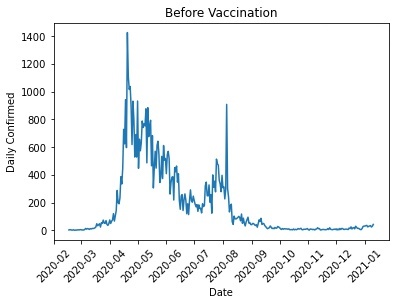
\includegraphics[scale = 0.5]{Final/ode model/before-2.jpg}
	\caption{Daily Confirmed before vaccination}
	\label{sir0}
\end{figure}
\begin{figure}
	\centering
	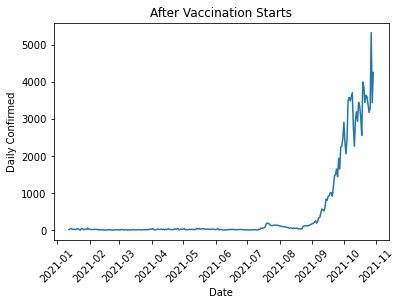
\includegraphics[scale = 0.5]{Final/ode model/after.jpg}
	\caption{Daily Confirmed after vaccination}
	\label{sir1}
\end{figure}
As the daily confirmed infectious data shows, there are mainly three outbreaks: the first peaks around May 2020, and the second starts from September 2021.

The outbreak around May 2020 according to the news report and the statistics data provided by the Ministry of Health (MOH) Singapore , happens mainly among the foreign workers who live in the crowded dorms. The outbreak starts from September 2021 is caused by Singapore's new policy that treats COVID-19 in the way of treating flu, including opening the board and canceling the guarantee requirements for specific travelers, which loosens the intervention upon the COVID-19 to a great extent and causes a wide spread in communities.

The first outbreak and the second outbreak happened in different vaccination and policy backgrounds. Thus if we want to get the effectiveness of vaccination upon the outbreak, at least we need to integrate the effectiveness of policy into my ODE equations.




\subsection{Model Description}
Because all infectious cases, including asymptomatic infectious cases and cases in incubation periods are also counted to the confirmed cases and are required isolation, we remove the exposed states in SEIR model and use the SIR model instead.

There are four compartments in our ODE model, with the Infectious comprising two states - Hospitalized and Isolated. Below is the flow among the compartments (See Figure \ref{sir2} and the ODE equations).
\begin{figure}
	\centering
	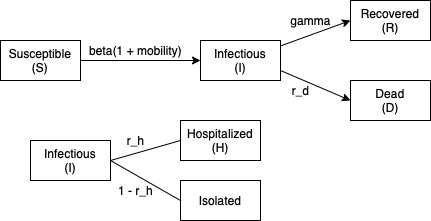
\includegraphics[scale = 0.5]{Final/ode model/ode model.jpg}
	\caption{Flow Diagram of our SIR model}
	\label{sir2}
\end{figure}
\begin{equation}
\begin{cases} ds/dt = -\beta S(t) I(t) (1 + mobility(t)/100)/N \\ di/dt = \beta s I(t) (1 + mobility(t)/100)/N - \gamma I(t) - (I) r_d\\ dd/dt = I(t) r_d \\ dh/dt = di/dt \times r_h\\ dr/dt = \gamma I(t) \end{cases}
\end{equation}

The Singapore COVID-19 dataset we get includes the basic datas that are related to the COVID-19 contamination in a region and its policies to intervene in the COVID-19. However data likes the exact number of confirmed infectious cases and the number of the hospitalized people are not enough to directly measure  specific states in ODE model. And due to factors like testing policies and statistical granularity, there might be inaccurate or missing data. Thus we researched Singapore's COVID-19 policies and the statistical report provided by the MOH and found proper statistical data for S, I, R states.

For the S states, I first set S =  Population - I - R.

For the I states, we set I  = Intensive Care Unit (ICU) + General Wards + In Isolation. This is the way MOH uses to calculate the number of the active infectious cases. And thanks to Singapore's strict social lockdown and tracking spread policies, this data is accurate enough to reflect the infectious situation.

For the R states, we set R = Cumulative Confirmed - Cumulative Death - I.



\subsection{ Model fitting}

We use the minimize function in lmfit module (Non-Linear Least-Squares Minimization and Curve-Fitting), which implements the Levenberg-Marquardt algorithm to minimize the error between the measured data and the fitted data.
At the start, we set the error as below, where $m$ indicates measured and $f$ indicates fitted.

\begin{equation}
\begin{split}
    error =\sum_{t}\bigl\{&(St_{m} - St_{f})^2+(It_{m} - It_{f})^2\\
    &+(Rt_{m} - Rt_{f})^2 +(Dt_{m} - Dt_{f})^2\bigr\}^{1/2}
\end{split}
\end{equation}

The problem within such residual can include:
\begin{itemize}
    \item Trying to minimize the error for fitting three curves at the same time leads to failure in every single curve.
    \item The absolute error for different curve is quite different. The value of S is much bigger than the value of I and the value of R thus it should allow bigger absolute error.
\end{itemize}

Thus we changed my fitting method to fit only one curve for one iteration. First we fit the Infectious curve, and then the death curve and the recovery curve.

After one iteration of fitting, we found it's hard to fit the infectious curve because the rate of Suspicious almost remains unchanged due to the sparsity of infectious case and the strict social lockdown policy in Singapore. With the s / N remains approximately 1, di/dt = beta * i (1+ mobile[t]) - gamma * i - rd * i and whether di/dt > 0 or di/dt < 0  is only influenced by mobile[t] (The mobility data is shown in Figure \ref{sir3} and \ref{sir4}).
\begin{figure}
	\centering
	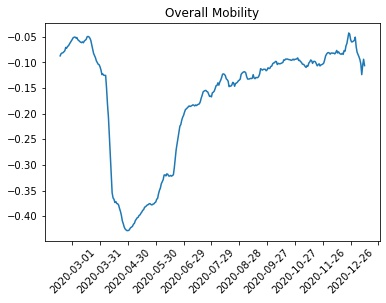
\includegraphics[scale = 0.5]{Final/ode model/mobility before.jpg}
	\caption{Mobility Before Vaccination}
	\label{sir3}
\end{figure}
\begin{figure}
	\centering
	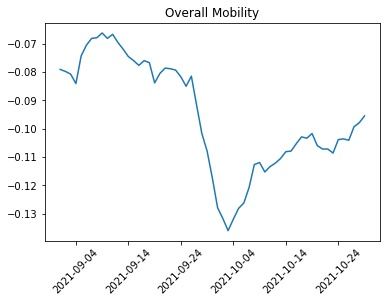
\includegraphics[scale = 0.5]{Final/ode model/mobility after.jpg}
	\caption{Mobility After Vaccination}
	\label{sir4}
\end{figure}

So after reading some papers who fit SEIR and SIR model to the real dataset, we decide to narrow the clique of COVID-19 spread in Singapore and set the total number of people rather than the population of Singapore, but instead as 110000 who are possible to engage in the spread and the number of the susceptible as 90000, and get a good fit.

\subsection{Observations}
As the fit results indicate, the beta of the first outbreak (May 2020) is 0.44964359, while the beta of the second outbreak (September 2021) is 0.18322612. With a more loose overall policy, the second outbreak still gain a better beta, which indicates that the vaccine has effectively prevented the spread of COVID-19.







